\section{Auswertung}
Zur quantitativen Auswertung der aufgenommenen RTM Bilder wird die Software \emph{gwyddion}\cite{gwyddion}
verwendet. Hiermit wird vorallem eine Rauschunterdrückung in den Aufnahmen durchgeführt und das Höhenprofil
der Goldprobe vermessen. Die Auswertungen der foreward und backward Scans erfolgen zunächst unabhängig, sodass
abschließend über die gewonnen Ergebnisse gemittelt werden kann.
Von einer quantitativen Analyse der im up Modus aufgenommen Bilder wird abgesehen. In Abbildung \ref{fig: up} ist eine
beispielhafte Aufnahme einzusehen. Hierauf ist klar zu erkennen, dass die Struktur stark verzerrt ist.
\begin{figure}
  \centering
  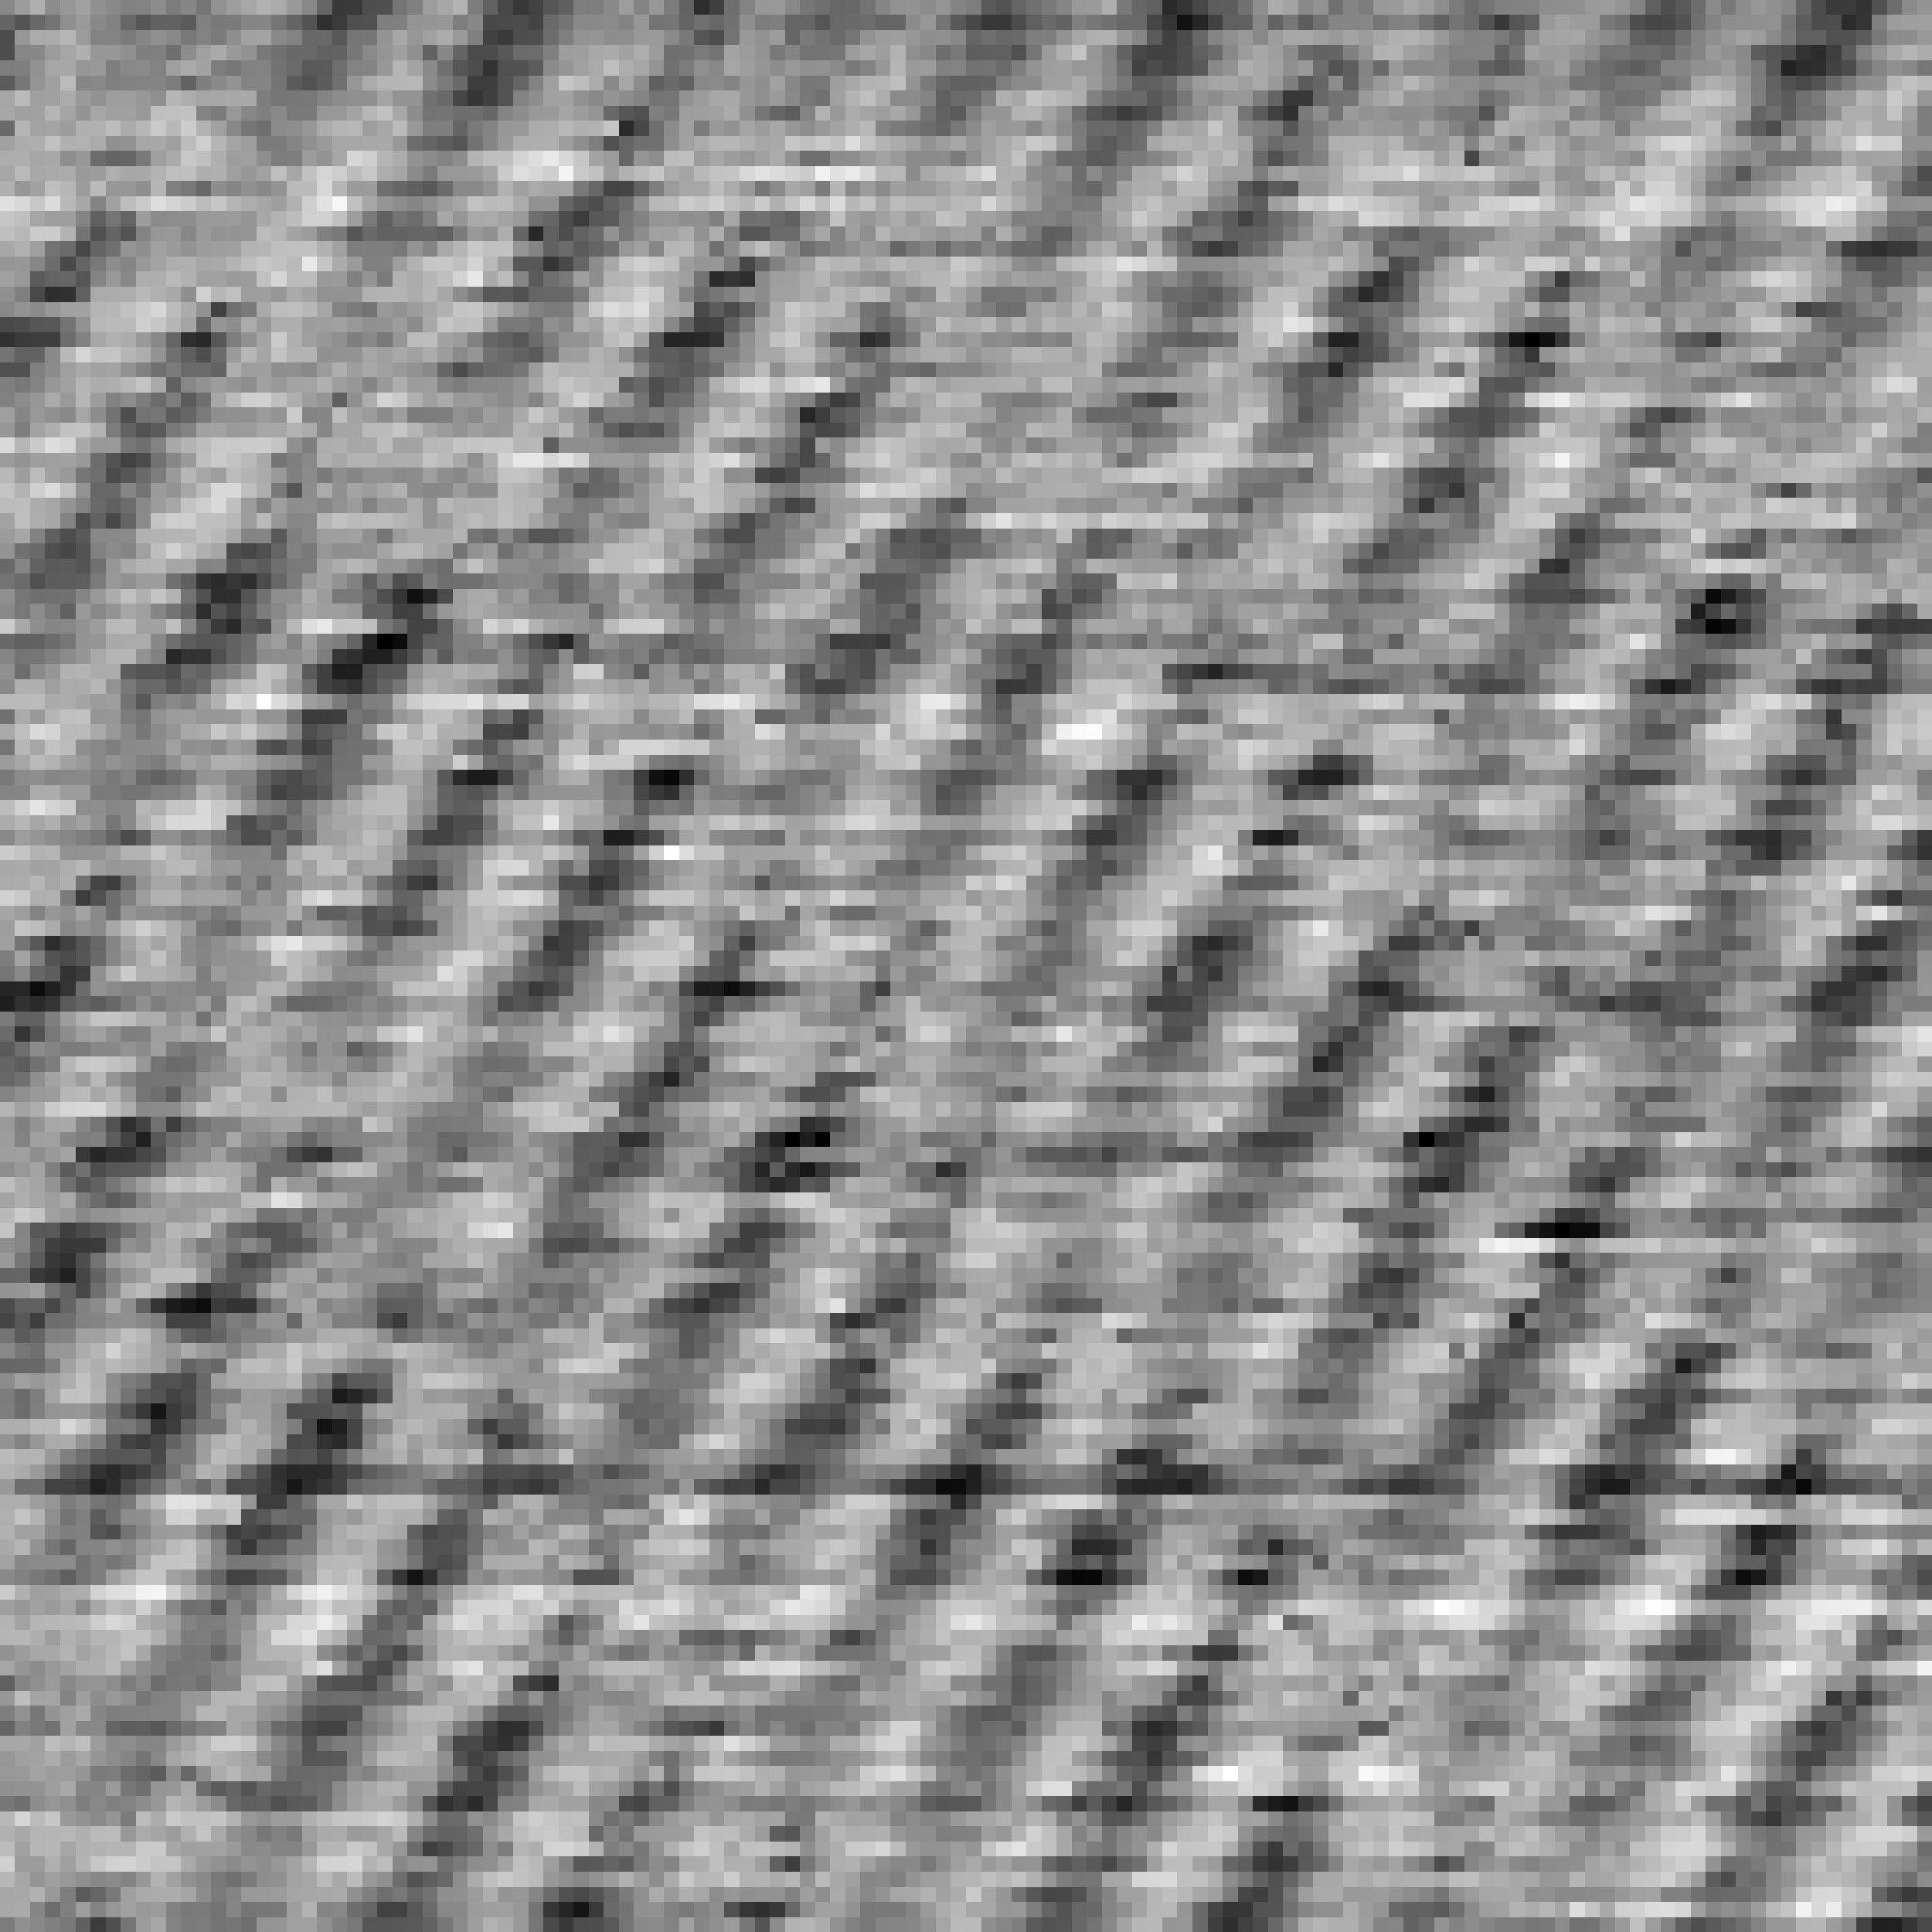
\includegraphics[width = 0.5\textwidth]{../Messdaten/bilder/up.png}
  \caption{RTM Aufnahme im up Modus.}
  \label{fig: up}
\end{figure}

\subsection{Untersuchung der HOPG-Probe}
Die aufgenommenen Bilder der HOPG-Probe im foreward und backward Modus sind in den Abbildungen~\ref{fig: foreward}
und~\ref{fig: backward} einzusehen.
\begin{figure}
  \centering
  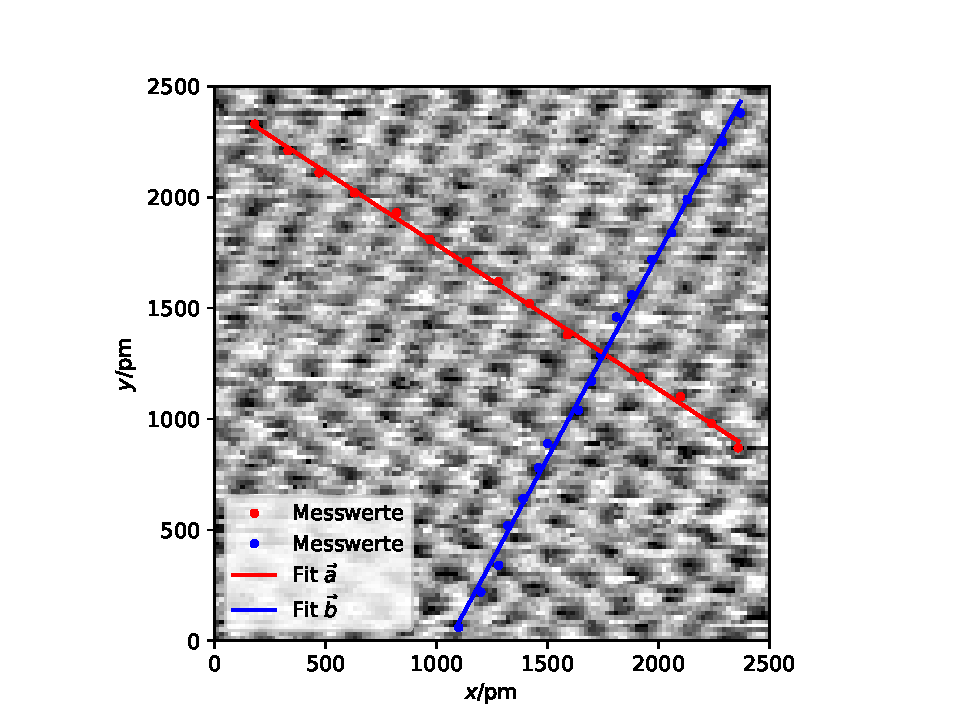
\includegraphics[width = \textwidth]{../Messdaten/bilder/fit_01_foreward.pdf}
  \caption{Foreward Scan der HOPG-Probe mit eingezeichneten Messwerten und linearen Regressionen.}
  \label{fig: foreward}
\end{figure}
\begin{figure}
  \centering
  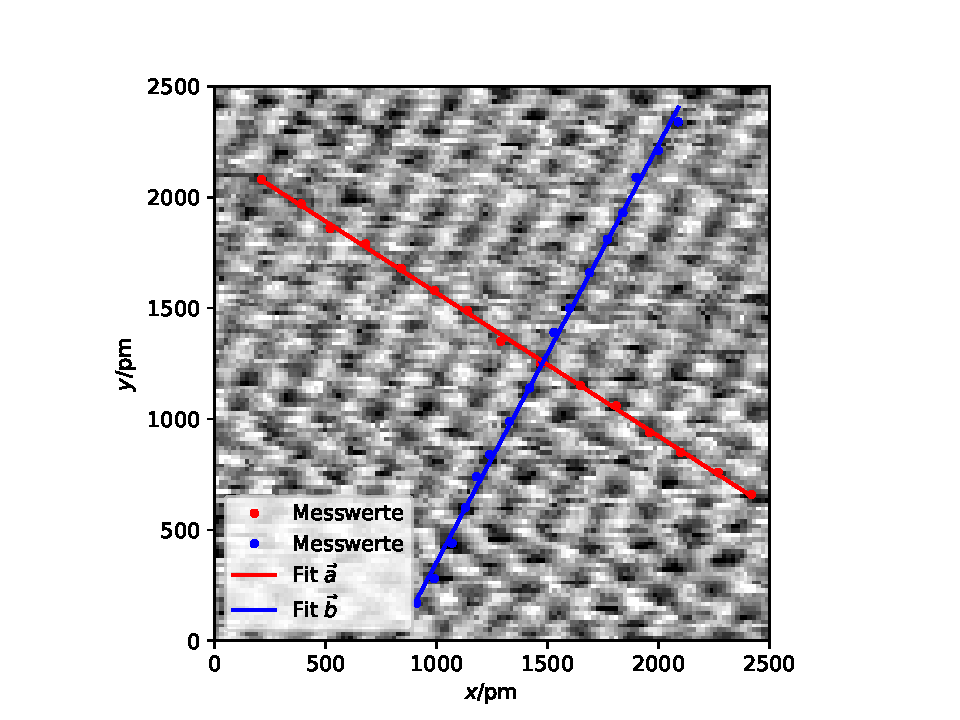
\includegraphics[width = \textwidth]{../Messdaten/bilder/fit_01_backward.pdf}
  \caption{Backward Scan der HOPG-Probe mit eingezeichneten Messwerten und linearen Regressionen.}
  \label{fig: backward}
\end{figure}
Entlang zweier Achsen $\vec{a}$ und $\vec{b}$ werden die Koordinaten der ersichtlichen Helligkeitsminima
abgelesen. Die Daten sind in Tabelle \ref{tab: data} eingetragen. Hiermit wird eine Regression an eine
lineare Funktion der Form
\begin{equation}
  y = m \cdot x + g
\end{equation}
durchgeführt.
\begin{table}
\centering
\caption{Aus den Scans bestimmte Koordinaten zur Regression an die Gittervektoren $\vec{a}$ und $\vec{b}$.}
\label{tab: data}
\begin{tabular}{S S S S S S S S}
\toprule
\multicolumn{4}{c}{Foreward} & \multicolumn{4}{c}{Backward} \\
{$x_{\vec{a}} / \si{\nano\meter}$} & {$y_{\vec{a}} / \si{ \nano\meter}$} & {$x_{\vec{b}} / \si{ \nano\meter}$} & {$y_{\vec{b}} / \si{ \nano\meter}$} & {$x_{\vec{a}} / \si{ \nano\meter}$} & {$y_{\vec{a}} / \si{ \nano\meter}$} & {$x_{\vec{b}} / \si{ \nano\meter}$} & {$y_{\vec{b}} / \si{ \nano\meter}$} \\
\midrule
0.18 & 2.33 & 1.10 & 0.06 & 0.21 & 2.08 & 0.91 & 0.17\\
0.33 & 2.21 & 1.20 & 0.22 & 0.39 & 1.97 & 0.99 & 0.28\\
0.47 & 2.11 & 1.28 & 0.34 & 0.52 & 1.86 & 1.07 & 0.44\\
0.63 & 2.02 & 1.32 & 0.52 & 0.68 & 1.79 & 1.13 & 0.60\\
0.82 & 1.93 & 1.39 & 0.64 & 0.84 & 1.68 & 1.18 & 0.74\\
0.97 & 1.81 & 1.46 & 0.78 & 0.99 & 1.58 & 1.24 & 0.84\\
1.14 & 1.71 & 1.50 & 0.89 & 1.14 & 1.49 & 1.33 & 0.99\\
1.28 & 1.62 & 1.64 & 1.04 & 1.29 & 1.35 & 1.42 & 1.14\\
1.42 & 1.52 & 1.70 & 1.17 & 1.47 & 1.25 & 1.48 & 1.26\\
1.59 & 1.38 & 1.74 & 1.29 & 1.65 & 1.15 & 1.53 & 1.39\\
1.75 & 1.29 & 1.81 & 1.46 & 1.81 & 1.06 & 1.60 & 1.50\\
1.92 & 1.19 & 1.88 & 1.56 & 1.96 & 0.94 & 1.69 & 1.66\\
2.10 & 1.10 & 1.97 & 1.72 & 2.10 & 0.85 & 1.77 & 1.81\\
2.24 & 0.98 & 2.06 & 1.84 & 2.27 & 0.76 & 1.84 & 1.93\\
2.36 & 0.87 & 2.13 & 1.99 & 2.42 & 0.66 & 1.90 & 2.09\\
 &  & 2.20 & 2.12 &  &  & 2.00 & 2.21 \\
 &  & 2.29 & 2.25 &  &  & 2.09 & 2.34 \\
 &  & 2.37 & 2.38 &  &  &  &  \\
\bottomrule
\end{tabular}
\end{table}


Die Fitparameter für foreward (f) und backward (b) Scan ergeben sich zu
\begin{align}
  m\ua{f, \vec{a}} &= \num{-0.652(7)} & g\ua{f, \vec{a}} &= \SI{2.44(1)}{\nano\meter} \\
  m\ua{f, \vec{b}} &= \num{1.85(3)} & g\ua{f, \vec{b}} &= \SI{-1.95(5)}{\nano\meter}
\end{align}
und
\begin{align}
  m\ua{b, \vec{a}} &= \num{-0.645(5)} & g\ua{b, \vec{a}} &= \SI{2.213(8)}{\nano\meter} \\
  m\ua{b, \vec{b}} &= \num{1.88(2)}   & g\ua{b, \vec{b}} &= \SI{-1.53(4)}{\nano\meter}
\end{align}
Die verwendeten Daten und Regressionsgeraden sind ebenfalls in den Abbildungen~\ref{fig: foreward}
und~\ref{fig: backward} eingezeichnet.
Die auftretenden Fehler der Regressionsrechnung liegen in einer Größenordnung, die außerhalb der Ablesegenauigkeit der
gefundenen Daten \ref{tab: data} liegt. Von einer Fortpflanzung der Fehler wird daher abgesehen. In der Diskussion
wird hierauf näher eingegangen.
Mit den Fitparamtern und den Koordinaten der ersten und letzten Punkte der abgelesenen Daten werden Gittervektoren $\vec{a}\ua{f, n_1}$, $\vec{b}\ua{f, n_2}$ und
$\vec{a}\ua{b, n_3}$, $\vec{b}\ua{b, n_4}$ bestimmt, die sich über $n\ua{i}$ Einheitszellen erstrecken
\begin{align}
  \vec{a}\ua{f, 14} &= \begin{pmatrix} \num{-2.18} \\  \num{1.42} \end{pmatrix}\si{\nano\meter} & \vec{b}\ua{f, 17}   &= \begin{pmatrix} \num{1.27} \\ \num{2.35} \end{pmatrix} \si{\nano\meter}\\
  \vec{a}\ua{b, 14} &= \begin{pmatrix}  \num{-2.21} \\ \num{1.43} \end{pmatrix}\si{\nano\meter} &  \vec{b}\ua{b, 16} &= \begin{pmatrix} \num{1.18} \\ \num{2.22} \end{pmatrix} \si{\nano\meter}.
\end{align}
Im Mittel ergeben sich folgende Gittervektoren $\vec{a}$ und $\vec{b}$ bezogen auf die Einheitszelle:
\begin{equation}
  \vec{a} = \begin{pmatrix} \num{-1.57(2)} \\  \num{1.017(2)} \end{pmatrix}\si{\angstrom} \qquad
  \vec{b} = \begin{pmatrix} \num{0.742(7)} \\  \num{1.384(5)} \end{pmatrix}\si{\angstrom}
\end{equation}
Mit den Beträgen
\begin{equation}
  \left|\vec{a}\right| = \SI{1.87(1)}{\angstrom} \quad \left|\vec{b}\right| = \SI{1.571(5)}{\angstrom}.
  \label{eq: mittlere_gittervektoren}
\end{equation}
und dem Innenwinkel:
\begin{equation}
  \theta = \SI{85.2(4)}{\degree}.
\end{equation}
Der Literaturwert für die Gitterkonstante $G$ beträgt gemäß \cite{} $G = \SI{2.56}{\angstrom}$. Zur quantitativen Analyse
der durch den Aufbau verzerrten Darstellung der Struktur sollen die Elemente einer Skalierungsmatrix $S$ ermittelt werden, die
die gefundenen Vektoren in die theoretischen Gittervektoren überführen soll. $S$ wird als diagonal angesetzt
\begin{equation}
  \vec{a}\ua{lit} = \begin{pmatrix} s\ua{x} & 0 \\  0  &   s\ua{y} \end{pmatrix} \vec{a},
  \qquad \vec{b}\ua{lit} = \begin{pmatrix} s\ua{x} & 0 \\  0  &   s\ua{y} \end{pmatrix} \vec{b}.
\end{equation}
Aus der der Forderung $G = \left|S \vec{a}\right| = \left|S \vec{b}\right|$ können die konstanten $s_x$ und $s_y$ ermittelt werden
\begin{align}
  s_y^2 &= \frac{G^2\left( a\ua{x}^2 - b\ua{x}^2\right)}{a\ua{x}^2 b\ua{y}^2 - a\ua{y}^2 b\ua{x}^2} \\
  s_x^2 &= \frac{G^2 - s\ua{y}^2 a\ua{y}^2}{a\ua{x}^2}.
\end{align}
Einsetzen der Werte der in \eqref{eq: mittlere_gittervektoren} aufgeführten Vektoren liefert
\begin{equation}
  s\ua{x} = \num{1.14(1)}  \qquad s\ua{y} = \num{1.670(8)}.
\end{equation}
Somit ergeben sich die skalierten Vektoren $\vec{a}\ua{skaliert}$ und $\vec{b}\ua{skaliert}$ zu
\begin{equation}
  \vec{a}\ua{skaliert} = \begin{pmatrix} \num{-1.780(8)} \\  \num{1.698(9)} \end{pmatrix}\si{\angstrom} \qquad
  \vec{b}\ua{skaliert} = \begin{pmatrix} \num{0.84(1)} \\  \num{2.311(5)} \end{pmatrix}\si{\angstrom}
\end{equation}
Der Winkel $\theta\ua{skaliert}$ zwischen den skalierten Vektoren beträgt.
\begin{equation}
  \theta\ua{skaliert} = \SI{66.4(6)}{\degree}.
\end{equation}


\subsection{Untersuchung der Goldprobe}
Das aufgenommene RTM Bild zur Untersuchung der Goldoberfläche ist in Abbildung~\ref{fig: au} einzusehen.
In der Abbildung ist zudem eine Gerade eingezeichnet entlang derer das Höhenprofil vermessen werden soll.
Die mit \emph{gwyddion} entnommenen Daten sind in Abbildung~\ref{fig: höhenprofil}
graphisch dargestellt. Gemäß den eingezeichneten vertikalen Linien
in Abbildung~\ref{fig: höhenprofil} werden die Daten zwei verschiedenen
Niveaus $h_1$ und $h_2$ zugeordnet, an denen eine Ausgleichsrechnung durchgeführt wird. Es ergeben sich für die
Niveaus
\begin{equation}
  h_1 = \SI{-58.180(7)}{\nano\meter} \qquad h_2 = \SI{-58.655(5)}{\nano\meter}
\end{equation}
Für die Höhendifferenz $\Delta h$ gilt damit
\begin{equation}
  \Delta h = \SI{4.75(9)}{\angstrom}.
\end{equation}
\begin{figure}
  \centering
  \includegraphics[width = 0.8\textwidth]{../Messdaten/bilder/goldoberfläche.pdf}
  \caption{Aufgenommenes RTM Bild der Goldoberfläche. Eingezeichnet ist die Linie entlang derer
  das Höhenprofil quantitativ untersucht wird.}
  \label{fig: au}
\end{figure}
\begin{figure}
  \centering
  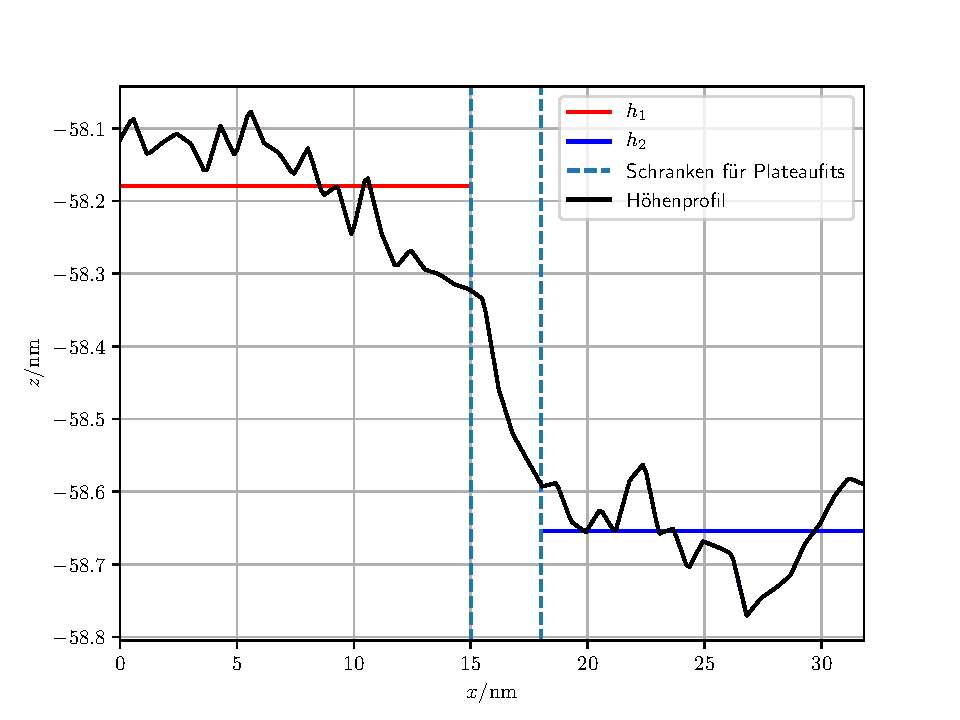
\includegraphics[width = 0.8\textwidth]{../Messdaten/bilder/au_plateau.pdf}
  \caption{Darstellung der Plateaus auf der Goldoberfläche. Eingezeichnet sind die Regressionen an
  konstante Werte der Höhe $z$.}
  \label{fig: höhenprofil}
\end{figure}
